\documentclass[twocolumn,english]{article}
\usepackage[latin9]{inputenc}
\usepackage[landscape]{geometry}
\geometry{verbose,tmargin=0.5in,bmargin=0.75in,lmargin=0.5in,rmargin=0.5in}
\setlength{\parskip}{0bp}
\setlength{\parindent}{0pt}
\usepackage{array}
\usepackage{float}
\usepackage{booktabs}
\usepackage{amsmath}
\usepackage{graphicx}

\makeatletter

\providecommand{\tabularnewline}{\\}




\usepackage{array}
\usepackage{multirow}
\usepackage{amsbsy}




\providecommand{\tabularnewline}{\\}

\setlength{\columnsep}{0.25in}
\usepackage{xcolor}
\usepackage{textcomp}
\usepackage{listings}
\lstset{
  tabsize=2,
  basicstyle=\small\ttfamily,
}



\usepackage{babel}
\usepackage{listings}
\renewcommand{\lstlistingname}{Listing}

\makeatother

\usepackage{babel}
\begin{document}

\title{Reference Sheet for CO231 Artificial Intelligence}

\date{Autumn 2017}
\maketitle

\section{Search}

\paragraph{Requirements}
\begin{enumerate}
\item \emph{Observable}: current state is known.
\item \emph{Discrete}: finitely many next states from each state.
\item \emph{Deterministic}: each action has exactly one outcome.
\item \emph{Known}: possible actions and next states known.
\end{enumerate}

\paragraph{Formal Definition}
\begin{enumerate}
\item Initial state (\emph{start}).
\item Transition model between states (\emph{graph}).
\item Goal tests (set of \emph{goal} states).
\item Path cost (sum of positive step costs).
\end{enumerate}
\rule[0.5ex]{0.25\columnwidth}{0.5pt}
\begin{enumerate}
\item Solution is \emph{path} from initial state to a goal state.
\item Optimal solution has lowest cost.
\end{enumerate}

\paragraph{Algorithms}

Generate a search tree:
\begin{enumerate}
\item Initialise the tree with initial state as root.
\item Repeat:
\begin{enumerate}
\item If frontier of tree is empty then fail.
\item Choose and remove leaf node $L$ from frontier.
\item If $L$ is a goal state, then return solution.
\item Add $L$ to seen states.
\item Expand $L$ (if not seen), adding resulting nodes to frontier.
\end{enumerate}
\end{enumerate}
To add \emph{loop checking}, each seen $L$ is added to an explored
set and only expanded if not already seen.

\paragraph{Uninformed / Blind Search}

Choose next unexpanded node using:
\begin{enumerate}
\item \emph{Breadth first search}: choose shallowest node.
\item \emph{Uniform cost search}: choose node with lowest path cost.
\item \emph{Depth first search}: choose deepest node.
\item \emph{Depth limited search}: DFS with depth limit $l$.
\item \emph{Iterative deepening search}: depth limited search with increasing
$l$.
\end{enumerate}
Variants:
\begin{enumerate}
\item \emph{Backtracking search}: only generate one node when expanded,
remember what to generate next.
\item \emph{Bi-directional search}: Two simultaneous searches from start
to goal and goal to start.
\end{enumerate}
Properties:
\begin{enumerate}
\item \emph{Completeness:} do we always find a solution if one exists?
\item \emph{Time complexity}: number of nodes expanded.
\item \emph{Space complexity}: max number of nodes in memory.
\item \emph{Optimality}: do we always find the least-cost solution?
\end{enumerate}
\begin{table}[H]
\centering{}%
\begin{tabular}{>{\centering}m{0.12\columnwidth}>{\centering}m{0.18\columnwidth}>{\centering}m{0.18\columnwidth}>{\centering}m{0.18\columnwidth}>{\centering}m{0.18\columnwidth}}
\toprule 
 & \textbf{\footnotesize{}Completeness} & \textbf{\footnotesize{}Time Complexity} & \textbf{\footnotesize{}Space Complexity} & \textbf{\footnotesize{}Optimality}\tabularnewline
\midrule
\emph{\footnotesize{}BFS} & {\footnotesize{}Yes if $b$ is finite} & {\footnotesize{}$O\left(b^{d}\right)$} & {\footnotesize{}$O\left(b^{d}\right)$} & {\footnotesize{}Yes if costs are constant}\tabularnewline
\addlinespace[0.25cm]
\emph{\footnotesize{}Uniform-cost} & {\footnotesize{}Yes if $b$ is finite and all costs are positive} & {\footnotesize{}$O\left(b^{d+1}\right)$ if costs are constant} & {\footnotesize{}$O\left(b^{d+1}\right)$ if costs are constant} & {\footnotesize{}Yes}\tabularnewline
\addlinespace[0.25cm]
\emph{\footnotesize{}DFS} & {\footnotesize{}Yes if $s$ is finite}\\
{\scriptsize{}(No without loop checking)} & {\footnotesize{}$s$}\\
{\scriptsize{}($O(b^{m})$ without loop checking)} & {\footnotesize{}$O\left(bm\right)$} & {\footnotesize{}No}\tabularnewline
\addlinespace[0.25cm]
\emph{\footnotesize{}Back-tracking DFS} & \multicolumn{4}{c}{{\footnotesize{}As for DFS but with $O\left(m\right)$ space complexity.}}\tabularnewline
\addlinespace[0.25cm]
\emph{\footnotesize{}Depth-limited DFS} & {\footnotesize{}No} & {\footnotesize{}$s\left(l\right)$}\\
{\scriptsize{}($O(b^{l})$ without loop checking)} & {\footnotesize{}$O\left(bl\right)$} & {\footnotesize{}No}\tabularnewline
\addlinespace[0.25cm]
\emph{\footnotesize{}Iterative deepening DFS} & \multicolumn{4}{c}{{\footnotesize{}As for BFS but with $O\left(bd\right)$ space complexity.}}\tabularnewline
\addlinespace[0.25cm]
\emph{\footnotesize{}Bidirectional BFS} & \multicolumn{4}{c}{{\footnotesize{}As for BFS but with $O\left(b^{d/2}\right)$ time
and space complexity.}}\tabularnewline
\bottomrule
\addlinespace[0.25cm]
\end{tabular}
\end{table}

Where:
\begin{itemize}
\item $b$ is the maximum branching factor of the search tree.
\item $d$ is the depth of the optimal solution.
\item $m$ is the max depth of the state space.
\item $s$ is the overall size of the state space.
\item $s\left(l\right)$ is the size of the state space up to depth $l$.
\end{itemize}

\paragraph{Informed / Heuristic-Based Search}

Use a cost estimate to choose node with least-estimated path cost.
\begin{enumerate}
\item \emph{Greedy-best-first-search}: $\text{cost estimate}=\text{heuristic on this node}$.
\item \emph{A{*} search}: $\text{cost estimate}=\text{actual cost to node}+\text{heuristic on this node}$.
\item \emph{Local search}: e.g. genetic algorithms, simulated annealing.
\end{enumerate}
Properties of heuristic functions (where $g\left(n,m\right)$ is the
actual cost of reaching $m$ from $n$ and $h\left(n\right)$ is the
heuristic applied to $n$:
\begin{enumerate}
\item \emph{Consistent} / \emph{Monotonic}: $h\left(n\right)\leq g\left(n,n'\right)+h\left(n'\right)$
for any $n'$ successor of $n$. (Doesn't overestimate actual cost
to any successor + heuristic applied to that node).
\item \emph{Admissible} (follows from consistency): $h\left(n\right)\leq g\left(n,m_{goal}\right)$
where $m_{goal}$ is the cheapest reachable goal from $n$. (Doesn't
overestimate actual cost to goal).
\end{enumerate}
\begin{itemize}
\item Often admissible / consistent heuristics come from a relaxed version
of the search problem (more edges).
\end{itemize}
Properties:

\begin{table}[H]
\centering{}%
\begin{tabular}{>{\centering}m{0.25\columnwidth}>{\centering}m{0.3\columnwidth}>{\centering}m{0.3\columnwidth}}
\toprule 
 & \textbf{\footnotesize{}Completeness} & \textbf{\footnotesize{}Optimality}\tabularnewline
\midrule
\emph{\footnotesize{}Greedy} & {\footnotesize{}Yes if $s$ is finite} & {\footnotesize{}No}\tabularnewline
\emph{\footnotesize{}Greedy (without loop checking)} & {\footnotesize{}No} & {\footnotesize{}No}\tabularnewline
\midrule
\emph{\footnotesize{}A{*}} & {\footnotesize{}Yes if $b$ is finite and all costs are positive} & {\footnotesize{}Yes if heuristic is consistent}\tabularnewline
\emph{\footnotesize{}A{*} (without loop checking)} & {\footnotesize{}Yes if $b$ is finite and all costs are positive} & {\footnotesize{}Yes if heuristic is admissible}\tabularnewline
\bottomrule
\end{tabular}
\end{table}

A{*} is optimally efficient but often runs out of space.

\paragraph{Adversarial Search}

Used for:
\begin{itemize}
\item Competitive environment (opponents with conflicting goals).
\item Unpredictable opponent.
\item Hard to solve, time limits.
\end{itemize}
Definitions for two-player, zero-sum games:
\begin{itemize}
\item $s_{0}$: initial state.
\item $\texttt{PLAYER}\left(s\right)$: which player moves in a state.
\item $\texttt{ACTIONS}\left(s\right)$: set of legal moves in a state.
\item $\texttt{RESULT}\left(s,a\right)$: state resulting from move in a
state.
\item $\texttt{UTILITY}\left(s,p\right)$: win (1), lose (-1) or draw (0).
\end{itemize}
Optimal strategies for perfect-information, deterministic games:
\begin{enumerate}
\item Minimax.
\item Alpha-beta pruning.
\end{enumerate}
Minimax:

\texttt{}
\begin{table}[H]
\raggedright{}\texttt{\small{}if $\lnot\texttt{TERMINAL}\left(s\right)$:}~\\
\texttt{\small{}$\qquad$if $\texttt{PLAYER}\left(s\right)=\texttt{MAX}$
then return $\max_{a=\texttt{ACTIONS}\left(s\right)}\texttt{MINIMAX}\left(\texttt{RESULT}\left(s,a\right)\right)$}~\\
\texttt{\small{}$\qquad$if $\texttt{PLAYER}\left(s\right)=\texttt{MIN}$
then return $\min_{a=\texttt{ACTIONS}\left(s\right)}\texttt{MINIMAX}\left(\texttt{RESULT}\left(s,a\right)\right)$}~\\
\texttt{\small{}if $\texttt{TERMINAL}\left(s\right)$:}~\\
\texttt{\small{}$\qquad$return $\texttt{UTILITY}\left(s\right)$}
\end{table}

Alpha-beta pruning:
\begin{itemize}
\item $\alpha$ is the minimum value that \texttt{MAX} is guaranteed to
achieve so far (minimiser's best guaranteed score).
\item $\beta$ is the maximum value that \texttt{MAX} is a guaranteed to
achieve so far (maximiser's best guaranteed score).
\end{itemize}
Starting with $\texttt{max-value}\left(s,-\infty,\infty\right)$:

\texttt{}
\begin{table}[H]
\raggedright{}\texttt{\small{}max-value$\left(s,\alpha,\beta\right)$:}~\\
\texttt{\small{}$\qquad$if $\lnot\texttt{TERMINAL}\left(s\right)$:}~\\
\texttt{\small{}$\qquad\qquad$let $v=-\infty$}~\\
\texttt{\small{}$\qquad\qquad$for each $a$ in $\texttt{ACTIONS}\left(s\right)$:}~\\
\texttt{\small{}$\qquad\qquad\qquad$let $v=\max\left(v,\texttt{min-value}\left(\texttt{RESULT}\left(s,a\right),\alpha,\beta\right)\right)$}~\\
\texttt{\small{}$\qquad\qquad\qquad$if $v\geq\beta$ then return
$v$}~\\
\texttt{\small{}$\qquad\qquad\qquad$else let $\alpha=\max\left(\alpha,v\right)$}~\\
\texttt{\small{}$\qquad\qquad$return $v$}~\\
\texttt{\small{}$\qquad$if $\texttt{TERMINAL}\left(s\right)$:}~\\
\texttt{\small{}$\qquad\qquad$return $\texttt{UTILITY}\left(s\right)$}
\end{table}
\texttt{}
\begin{table}[H]
\raggedright{}\texttt{\small{}min-value$\left(s,\alpha,\beta\right)$:}~\\
\texttt{\small{}$\qquad$if $\lnot\texttt{TERMINAL}\left(s\right)$:}~\\
\texttt{\small{}$\qquad\qquad$let $v=\infty$}~\\
\texttt{\small{}$\qquad\qquad$for each $a$ in $\texttt{ACTIONS}\left(s\right)$:}~\\
\texttt{\small{}$\qquad\qquad\qquad$let $v=\min\left(v,\texttt{max-value}\left(\texttt{RESULT}\left(s,a\right),\alpha,\beta\right)\right)$}~\\
\texttt{\small{}$\qquad\qquad\qquad$if $v\leq\alpha$ then return
$v$}~\\
\texttt{\small{}$\qquad\qquad\qquad$else let $\beta=\min\left(\beta,v\right)$}~\\
\texttt{\small{}$\qquad\qquad$return $v$}~\\
\texttt{\small{}$\qquad$if $\texttt{TERMINAL}\left(s\right)$:}~\\
\texttt{\small{}$\qquad\qquad$return $\texttt{UTILITY}\left(s\right)$}
\end{table}
\begin{itemize}
\item \emph{Key idea}: If this move ever gives the opponent a choice to
do better than the best they could do in a different move, then we
shouldn't consider it.
\end{itemize}
Properties:

\begin{table}[H]
\centering{}%
\begin{tabular}{>{\centering}m{0.12\columnwidth}>{\centering}m{0.18\columnwidth}>{\centering}m{0.18\columnwidth}>{\centering}m{0.18\columnwidth}>{\centering}m{0.18\columnwidth}}
\toprule 
 & \textbf{\footnotesize{}Completeness} & \textbf{\footnotesize{}Time Complexity} & \textbf{\footnotesize{}Space Complexity} & \textbf{\footnotesize{}Optimality}\tabularnewline
\midrule
\emph{\footnotesize{}Minimax} & {\footnotesize{}Yes if search tree is finite} & {\footnotesize{}$O\left(b^{m}\right)$} & {\footnotesize{}$O\left(bm\right)$} & {\footnotesize{}Yes}\tabularnewline
\addlinespace[0.25cm]
\emph{\footnotesize{}$a$-$\beta$ pruning} & \multicolumn{4}{c}{{\footnotesize{}As for minimax but with $O\left(b^{m/2}\right)$ time
complexity.}}\tabularnewline
\bottomrule
\addlinespace[0.25cm]
\end{tabular}
\end{table}

Limited Resources:
\begin{itemize}
\item Cutoff-test instead of \texttt{TERMINAL}.
\item Evaluation instead of \texttt{UTILITY}.
\end{itemize}

\section{Planning}

\paragraph{Requirements}

Observable, discrete, deterministic, known.

\paragraph{STRIPS Language for Planning}
\begin{enumerate}
\item \emph{States} - conjunctions of ground atoms.
\item \emph{Goals} - conjunctions of literals - possibly containing variables
- implicitly existentially quantified.
\item \emph{Operators}:
\begin{enumerate}
\item Action description.
\item \emph{Precondition} - conjunction of literals.
\item \emph{Postcondition} (\emph{Effect}) - conjunction of literals. Every
variable in effect must appear in pre-condition.
\end{enumerate}
\item \emph{Actions} - fully instantiated operators.
\end{enumerate}
\[
\text{Precondition}\xrightarrow{\text{Action}}\text{Postcondition}
\]

\paragraph{Execution of an Action}

New State = Current state - negation of negative fluents in effects
+ positive fluents in effects

\paragraph{Assumptions}
\begin{itemize}
\item Fluents not mentioned in a state are false.
\item Fluents do not change unless they are explicitly changed by an action.
\item Time is implicit.
\end{itemize}

\paragraph{Planning as Search}
\begin{enumerate}
\item \emph{Progression planning} (forward) - blind search with the graph
obtained from the specification of the planning problem.
\begin{enumerate}
\item \emph{Problem}: Large search spaces with many irrelevant actions.
\item \emph{Solution}: Good heuristics; relax the problem, add extra edges
e.g. by ignoring preconditions and effects not in goal.
\end{enumerate}
\item \emph{Regression planning} (backward) - blind search backwards from
the goal.
\begin{enumerate}
\item \emph{Problem}: Non-interleaved regression planning is incomplete
\end{enumerate}
\end{enumerate}

\subsubsection*{Graph-Plan Algorithm}

\begin{figure}[H]
\centering{}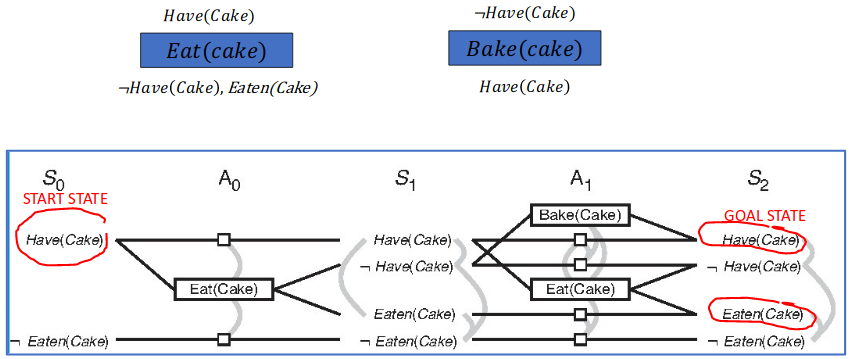
\includegraphics[width=0.9\columnwidth]{img/graph-plan}
\end{figure}
\begin{itemize}
\item \emph{Level $S_{i}$}:
\begin{itemize}
\item $i=0$: Start state + literals that could hold at the start.
\item $i>0$: all literals that could hold at $S_{i}$, depending on actions
at $A_{i-1}$.
\end{itemize}
\item \emph{Level $A_{i}$}:
\begin{itemize}
\item Each action in $A_{i}$ connected to its precondition in $S_{i}$
and effect at $S_{i+1}$.
\item No-op actions: no change.
\end{itemize}
\item Mutual exclusions between actions when:
\begin{itemize}
\item Actions have \emph{inconsistent effects}.
\item \emph{Interference}: effect of one action = $\lnot$ precondition
of the other.
\item \emph{Competing needs}: mutually exclusive pre-conditions.
\end{itemize}
\item Mutual exclusions between literals when:
\begin{itemize}
\item They are \emph{complementary}.
\item \emph{Inconsistent support}: Each possible pair of actions achieving
them are mutex.
\end{itemize}
\item Levelling off:
\begin{itemize}
\item When two consecutive levels are identical.
\end{itemize}
\end{itemize}

\paragraph{Extracting the Plan}

Once goal is non-mutex in $S_{i}$, search backwards to extract plan.
\end{document}
